\begin{figure}[H]
	\centering
	\begin{tikzpicture}
		\GraphInit[vstyle=Classic]
		\SetGraphUnit{2}
		\tikzset{EdgeStyle/.style={->,>=latex}}
		%\draw[help lines] (0,0) grid (9,2);
		\Vertex[x=0,y=0,Lpos=-90,L={$f_1$}]{f1}
		\Vertex[x=3,y=0,Lpos=-90,L={$f_2$}]{f2}
		\Vertex[x=6,y=0,Lpos=-90,L={$f_3$}]{f3}
		\Edge[label={$\direct{\varrho}{1}{2} \direct{\delta}{1}{2}$}](f1)(f2)
		\Edge[label={$\direct{\varrho}{2}{3} \direct{\delta}{2}{3}$}](f2)(f3)
	\end{tikzpicture}
	\caption{\ac{dag} of a three source linear hierarchy}
	\label{fig:min_lin}
\end{figure}
